\chapter{Higher Order Reconstruction Procedures}
\label{ap:reco}
\markboth{Higher Order Reconstruction Procedures}{}
\graphicspath{{image_directory/appendix/}}

\section{MUSCL}
\label{ap:MUSCLreco}

	For the single cell $i$, the left and right reconstructed states are given by $\rho^{R}_{i-1/2}$ and $\rho_{i+1/2}^{L}$ respectively. 

\subsection{Linear - 2nd Order}
	
	The 2nd order MUSCL scheme approximates the cell density distribution with a linear slope. The left and right states are given by
	\begin{align}
		\rho^{R}_{i-1/2}&=\rho_i-\frac{1}{2}\phi\left(r_i\right)\left(\rho_{i+1}-\rho_{i}\right),\\
		\rho^{L}_{i+1/2}&=\rho_i+\frac{1}{2}\phi\left(r_i\right)\left(\rho_{i+1}-\rho_{i}\right),
	\end{align}
	where 
	\begin{equation}
		r_{i}=\frac{\rho_{i}-\rho_{i-1}}{\rho_{i+1}-\rho_{i}},
	\end{equation}
	and $\phi$ is the slope limiting function.
	
	\begin{figure}
    		\centering
        		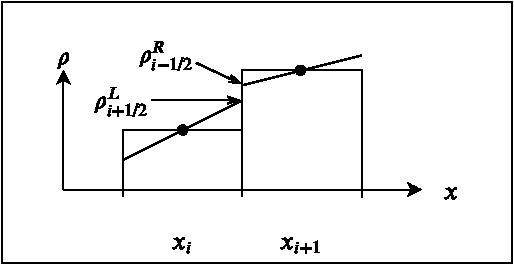
\includegraphics[trim=20 5 20 20,clip,width=0.6\textwidth]{MUSCL_linear.pdf}
		\caption[MUSCL Reconstruction : Linear $2^{nd}$ order]{MUSCL second order piecewise linear reconstruction.}
		\label{fig:app:muscl_lin}
	\end{figure}
	
\subsection{Parabolic - 3rd Order}

	The 3rd order MUSCL scheme approximates the cell density distribution with a parabolic slope, from a second order interpolation. The left and right states are given by
	\begin{align}
		\rho^{R}_{i-1/2}&=\rho_{i}-\frac{1}{4}\phi\left(r_{i}\right)\left[\left(1-\kappa\right)\delta\rho_{i+1/2}+\left(1+\kappa\right)\delta\rho_{i-1/2}\right],\\
		\rho^{L}_{i+1/2}&=\rho_{i}+\frac{1}{4}\phi\left(r_{i}\right)\left[\left(1-\kappa\right)\delta\rho_{i-1/2}+\left(1+\kappa\right)\delta\rho_{i+1/2}\right],
	\end{align}
	with $\kappa=1/3$, $\delta\rho_{i+1/2}=\rho_{i+1}-\rho_{i}$, $\delta\rho_{i-1/2}=\rho_{i}-\rho_{i-1}$, and the slope limiter $\phi$.
	
	\begin{figure}
    		\centering
        		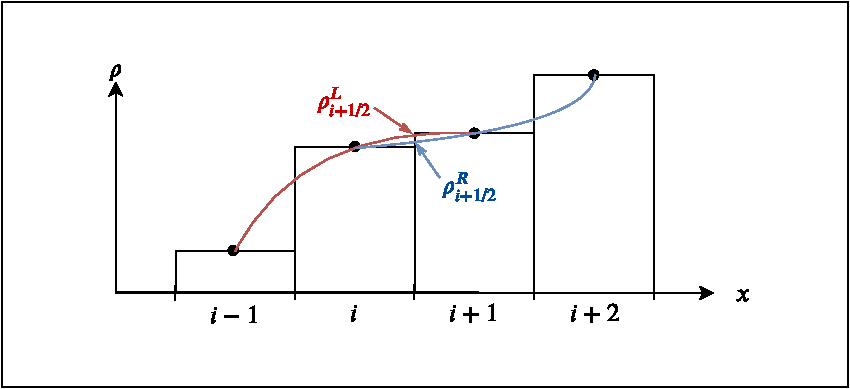
\includegraphics[trim=40 30 40 30,clip,width=0.7\textwidth]{MUSCL_para.pdf}
		\caption[MUSCL Reconstruction : Parabolic $3^{rd}$ order]{MUSCL third order piecewise parabolic reconstruction using second order interpolation.}
		\label{fig:app:muscl_para}
	\end{figure}
	
\subsection{Slope Limiters}
\label{ap:MUSCLslopelim}

	The listed slope limiters apply to MUSCL reconstructions to reduce cell interface oscillations. All present limiters are written in \emph{MUSCLReconstruction.py}, Appendix  \ref{code:musclreconstruction} [lines 90-185].
	
	\begin{itemize}
	
		\item CHARM [not 2nd order TVD] \cite{Zhou95}
			\begin{equation}
				\phi\left(r\right)=
				\begin{cases}
					\frac{r\left(3r+1\right)}{\left(r+1\right)^2},    &r>0\\
					0,  &r\leq0
				\end{cases}
			\end{equation}
			
		\item HCUS [not 2nd order TVD] \cite{Waterson95}
			\begin{equation}
				\phi\left(r\right)=\frac{3\left(r+\left|r\right|\right)}{2\left(r+2\right)}
			\end{equation}
			
		\item HQUICK [not 2nd order TVD] \cite{Waterson95}
			\begin{equation}
				\phi\left(r\right)=\frac{2\left(r+\left|r\right|\right)}{\left(r+3\right)}
			\end{equation}
			
		\item Koren [3rd order TDV accurate for sufficiently smooth data] \cite{Koren93}
			\begin{equation}
				\phi\left(r\right)=\max\left[0,\min\left(2r,\min\left(\frac{1+2r}{3},2\right)\right)\right]
			\end{equation}
			
		\item MinMod [2rd order TDV accurate] \cite{Roe86}
			\begin{equation}
				\phi\left(r\right)=\max\left[0,\min\left(1,r\right)\right]
			\end{equation}
			
		\item Monotonized Central (MC) [2rd order TDV accurate, symmetric] \cite{VanLeer77}
			\begin{equation}
				\phi\left(r\right)=\max\left[0,\min\left(2r, \frac{1+r}{2},2\right)\right]
			\end{equation}
			
		\item Osher [2rd order TDV accurate] \cite{Osher83}
			\begin{equation}
				\phi\left(r\right)=\max\left[0,\min\left(r,\beta\right)\right], \quad\left(1\leq\beta\leq2\right)
			\end{equation}
			
		\item Ospre [2rd order TDV accurate, symmetric] \cite{Waterson95}
			\begin{equation}
				\phi\left(r\right)=\frac{3\left(r^2+r\right)}{2\left(r^2+r+1\right)}
			\end{equation}
			
		\item Smart [not 2rd order TDV] \cite{Gaskell88}
			\begin{equation}
				\phi\left(r\right)=\max\left[0,\min\left(2r,\frac{1+3r}{4},4\right)\right]
			\end{equation}
			
		\item Superbee [2rd order TDV accurate, symmetric] \cite{Roe86}
			\begin{equation}
				\phi\left(r\right)=\max\left[0,\min\left(2r,1\right),\min\left(r,2\right)\right]
			\end{equation}
			
		\item Sweby [not 2rd order TDV, symmetric] \cite{Sweby84}
			\begin{equation}
				\phi\left(r\right)=\max\left[0,\min\left(\beta r,1\right),\min\left(r,\beta\right)\right], \quad\left(1\leq\beta\leq2\right)
			\end{equation}
			
		\item UMIST [2rd order TDV accurate] \cite{Lien94}
			\begin{equation}
				\phi\left(r\right)=\max\left[0,\min\left(2r,\frac{1+3r}{4},\frac{3+r}{4},2\right)\right]
			\end{equation}
			
			\newpage
			
		\item van Albada 1 [2rd order TDV accurate, symmetric] \cite{VanAlbada82}
			\begin{equation}
				\phi\left(r\right)=\frac{r^2+r}{r^2+1}
			\end{equation}
			
		\item van Albada 2 - alternate form for high spatial order schemes [not 2rd order TDV] \cite{Kermani03}
			\begin{equation}
				\phi\left(r\right)=\frac{2r}{r^2+1}
			\end{equation}
			
		\item van Leer [2nd order TVD accurate, symmetric] \cite{VanLeer74}
			\begin{equation}
				\phi\left(r\right)=\frac{r+\left|r\right|}{1+\left|r\right|}
			\end{equation}
	
	\end{itemize}
	
	\subsection*{Other Limiters}

	To calculate the gradient limiter, Barth and Jesperson \cite{Barth89} suggested using $\Phi_i=\min\left(\Phi_{ij}\right)$, where
	\begin{equation}
		\Phi_{ij}=
		\begin{cases}
			\min\left(1,\frac{\delta \rho_i^{\max}}{\rho_{ij}-\overline{\rho}_i}\right), & if \quad \rho_{ij}-\overline{\rho}_i>0, \\
			\min\left(1,\frac{\delta \rho_i^{\min}}{\rho_{ij}-\overline{\rho}_i}\right), & if \quad \rho_{ij}-\overline{\rho}_i<0,\\
			1, & if \quad \rho_{ij}-\overline{\rho}_i=0.
		\end{cases}
		\nonumber
	\end{equation}
	The values $\delta \rho_i^{\max}$ and $\delta \rho_i^{\min}$ are the maximum and minimum of $\overline{\rho}-\overline{\rho}_i$ respectively, the difference between the concerned volume and nearest neighbours. The value, $\rho_{ij}=R_i\left(\vec{x}_j-\vec{x}_i\right)$, is the unlimited reconstructed value. Due to the minimum, maximum, and case selections of $\Phi_i$ in the Barth and Jespersen limiter, the reconstructed flux is non-differentiable, which slows the solving convergence. Venkatakrishnan \cite{Venkatakrishnan93} suggested a smooth approximation of the case selection step in the Barth and Jespersen limiter. This approximation uses $\phi(r)$ instead of $\min(1,r)$, where 
	\begin{equation}
		\phi(r)=\frac{r^2+2r}{r^2+r+2}, \label{eq:ven_approx}
	\end{equation}
	so for $\rho_{ij}-\overline{\rho}_i<0$
	\begin{equation}
		\Phi_{ij}=\phi\left(\frac{\delta \rho_i^{\min}}{\rho_{ij}-\overline{\rho}_i}\right). \nonumber
	\end{equation}
	Venkatakrishnan also suggested avoiding the limiter for regions of uniform flow, i.e. when $\rho_{ij}-\overline{\rho}_i>0$
	\begin{equation}
		\Phi_{ij}=\frac{1}{\Delta_-}\left[\frac{\left(\Delta_+^2+\epsilon^2\right)\Delta_-+2\Delta_-^2\Delta_+}{\Delta_+^2+2\Delta_-^2+\Delta_-\Delta_++\epsilon^2}\right], \nonumber
	\end{equation}
	where $\Delta_-=\rho_{ij}-\overline{\rho}_i$, $\Delta_+=\delta \rho_i^{\max}$, and $\epsilon^2=\left(K\Delta x\right)^3$ with parameter $K>0$. The case for $\rho_{ij}-\overline{\rho}_i=0$ remains unchanged with $\Phi_{ij}=1$.
	
	\begin{figure}
    		\centering
        		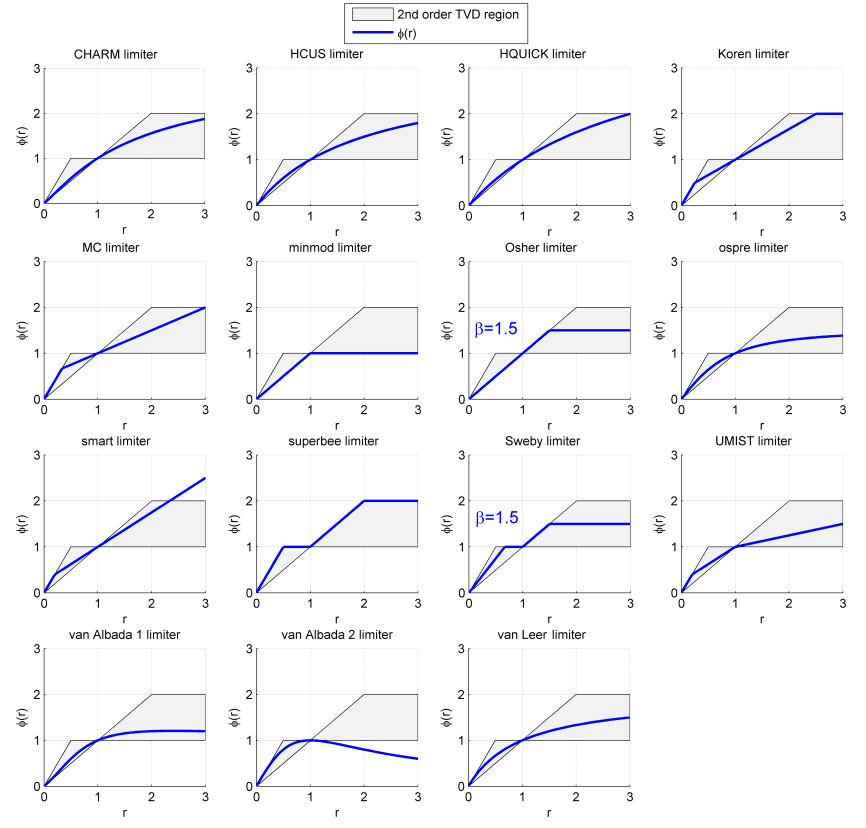
\includegraphics[trim=0 0 0 0,clip,width=\textwidth]{Limiters.png}
		\caption[MUSCL Reconstruction : Slope limiters]{Plots showing the slope limiter $\phi(r)$ on $r\geq0$ over the admissible TVD region for second order schemes \cite{Sweby84}. Created in MATLAB \cite{Griffgruff}.}
		\label{fig:app:slopelims}
	\end{figure}
	

\section{WENO}
\label{ap:WENOreco}

	The general $\left(2k-1\right)^{th}$ order WENO reconstruction considers a convex combination of $k$ reconstructions from unique local stencils. See \cite{Shu97} for a more thorough discussion and derivation of WENO and ENO schemes, Procedure 2.2 provides the general WENO scheme steps presented here. The available $3^{rd}$, $5^{th}$, and $7^{th}$ order reconstructions in \emph{WENOReconstruction.py} \ref{code:wenoreconstruction} are represented by $k=2,3,4$ respectively. For cell $i$, we want approximations for the left, $\rho^{+}_{i-1/2}$, and right, $\rho^{-}_{i+1/2}$, density values. The following steps provide an algorithm for computing the WENO reconstructed cell interface values to the required order.
\begin{enumerate}
	\item Consider the $k$ stencils over $x_{i-(k-1)},\hdots,x_{i+(k-1)}$, denoted by $S_r$ for $r=0,\hdots,k-1$,
		\begin{equation}
			S_r=\left\{x_{i-r}, x_{i-r+1},\hdots,x_{i-r+(k-1)}\right\}.
		\end{equation}
	\item Obtain $k$ \emph{right} and $k$ \emph{left} reconstructed values,
		\begin{equation}
			\rho^{(r)}_{i+1/2}=\sum_{j=0}^{k-1}c_{r,j}\overline\rho_{i-r+j},\quad\text{and},\quad \rho^{(r)}_{i-1/2}=\sum_{j=0}^{k-1}\tilde c_{r,j}\overline\rho_{i-r+j}
		\end{equation}
		using the cell averaged density values $\overline\rho$, and weights $c_{r,j}$ and $\tilde c_{r,j}$ with $\tilde c_{r,j}=c_{r-1,j}$ ($r=-1$ is provided for the left-right transformation purposes) where $c_{r,j}$ are
		\begin{center}
			\begin{tabular}{|c|c|cccc|}
				\hline
 				\multirow{2}{*}{$k$} & \multirow{2}{*}{$r$} & \multicolumn{4}{c|}{$j$} \\
 				 & & 0 & 1 & 2 & 3 \\
 				 \hline
 				\multirow{2}{*}{$2$} & -1 & 3/2 & -1/2 & - & - \\
 				& 0 & 1/2 & 1/2 & - & - \\
 				& 1 & -1/2 & 3/2 & - & - \\
 				 \hline
 				\multirow{3}{*}{$3$} & -1 & 11/6 & -7/6 & 1/3 & - \\
 				& 0 & 1/3 & 5/6 & -1/6 & - \\
 				& 1 & -1/6 & 5/6 & 1/3 & - \\
 				& 2 & 1/3 & -7/6 & 11/6 & - \\
 				\hline
 				\multirow{4}{*}{$4$} & -1 & 25/12 & -23/12 & 13/12 & -1/4 \\
 				& 0 & 1/4 & 13/12 & -5/12 & 1/12 \\
 				& 1 & -1/12 & 7/12 & 7/12 & -1/12 \\
 				& 2 & 1/12 & -5/12 & 13/12 & 1/4 \\
 				& 3 & -1/4 & 13/12 & -23/12 & 25/12 \\
 				\hline
			\end{tabular}
		\end{center}
	
	\item Define the constants $d_r$ and $\tilde d_r=d_{k-1-r}$
		\begin{center}
			\begin{tabular}{|c|ccc|}
				\hline
				\multirow{2}{*}{$r$} & \multicolumn{3}{c|}{$k$}\\
				& 2 & 3 & 4 \\
				\hline
				0 & 2/3 & 3/10 & 4/35\\
				1 & 1/3 & 3/5 & 18/35\\
				2 & - & 1/10 & 12/35\\
				3 & - & - & 1/35\\
				\hline
			\end{tabular}
		\end{center}
	
	\item Find the smoothness indicators. For $k=2$ these can be written in a simple form
		\begin{equation}
			\beta_r=\left(\overline\rho_{i+1-r}-\overline\rho_{i-r}\right)^2.
		\end{equation}
		The smoothness indicator form for $k=3$ is
		\begin{equation}
			\beta_r = \frac{13}{12}\left(\sum_{j=0}^{k-1}b^{(0)}_{r,j}\overline\rho_{i-r+j}\right)^2+\frac{1}{4}\left(\sum_{j=0}^{k-1}b^{(1)}_{r,j}\overline\rho_{i-r+j}\right)^2,
		\end{equation}
		with coefficients as below.
		\begin{center}
			\begin{tabular}{|c|ccc|ccc|}
				\hline
				 \multirow{2}{*}{$r$} & \multicolumn{3}{|c|}{$b^{(0)}$ : $j$} & \multicolumn{3}{|c|}{$b^{(1)}$ : $j$}\\
				 & 0 & 1 & 2 & 0 & 1 & 2\\
				 \hline
				 0 & 1 & -2 & 1 & 3 & -4 & 1\\
				 1 & 1 & -2 & 1 & 1 & 0 & -1\\
				 2 & 1 & -2 & 1 & 1 & -4 & 3\\
				\hline
			\end{tabular}
		\end{center}
		For higher order WENO schemes, the smoothness factors of which are of the form \cite{BalsaraShu00}
		\begin{equation}
			\beta_r = \sum^{k-1}_{j=0}\left[\overline\rho_{i-r+j}\cdot\left(\sum_{g=0}^{k-1-j}\hat{b}_{r,j,g}\cdot\overline\rho_{i-r+j+g}\right)\right]
		\end{equation}
		with $\hat{b}_{r,j,g}$ from
		\begin{center}
			\begin{tabular}{|c|c|cccc|}
			\hline
				 \multirow{2}{*}{$r$} & \multirow{2}{*}{$j$} & \multicolumn{4}{c|}{$g$} \\
				  & & 0 & 1 & 2 & 3 \\
			\hline
				 \multirow{4}{*}{$0$}  & 0 & 2107 & -9402 & 7042 & -1854 \\
				                                      & 1 & 11003 & -17246 & 4642 & - \\
				                                      & 2 & 7043 & -3882 & - & - \\
				                                      & 3 & 547 & - & - & - \\
			\hline
				 \multirow{4}{*}{$1$}  & 0 & 547 & -2522 & 1922 & -494 \\
				                                      & 1 & 3443 & -5966 & 1602 & - \\
				                                      & 2 & 2843 & -1642 & - & - \\
				                                      & 3 & 267 & - & - & - \\
			\hline
				 \multirow{4}{*}{$2$}  & 0 & 267 & -1642 & 1602 & -494 \\
				                                      & 1 & 2843 & -5966 & 1922 & - \\
				                                      & 2 & 3443 & -2522 & - & - \\
				                                      & 3 & 547 & - & - & - \\
			\hline
				 \multirow{4}{*}{$3$}  & 0 & 547 & -3882 & 4642 & -1854 \\
				                                      & 1 & 7043 & -17246 & 7042 & - \\
				                                      & 2 & 11003 & -9402 & - & - \\
				                                      & 3 & 2107 & - & - & - \\
			\hline
			\end{tabular}
		\end{center}
		using the cell averaged density values $\overline\rho$.
		
	\item[5a] Calculate alpha weights
		\begin{align}
			\tilde\alpha_r&=\frac{\tilde d_r}{\left(\epsilon+\beta_r\right)^2},\\
			\alpha_r&=\frac{d_r}{\left(\epsilon+\beta_r\right)^2},
		\end{align}
		using the weights $d$ from step 3, and the smoothness indicators $\beta$ from step 4. The constant $\epsilon=10^{-6}$ to avoid a division by zero.
		
	\item[5b] Calculate the omega weights
		\begin{align}
			\tilde\omega_r&=\frac{\tilde\alpha_r}{\tilde\alpha_0+\tilde\alpha_1+\tilde\alpha_2}, \\
			\omega_r&=\frac{\alpha_r}{\alpha_0+\alpha_1+\alpha_2},
		\end{align}
		using the weights $\alpha$ from step 5a.
		
	\item[6] Evaluate the final interface reconstructions
		\begin{align}
			\rho^{-}_{i+1/2}&=\sum_{j=0}^{k-1}\omega_j\rho^{(j)}_{i+1/2}, \\
			\rho^{+}_{i-1/2}&=\sum_{j=0}^{k-1}\tilde\omega_j\rho^{(j)}_{i-1/2},
		\end{align}
		using the weights $\omega$ from step 5b, and the polynomial reconstructed values $\rho_{i\pm1/2}^{(r)}$ from step 2.
\end{enumerate}

	\begin{figure}
    		\centering
        		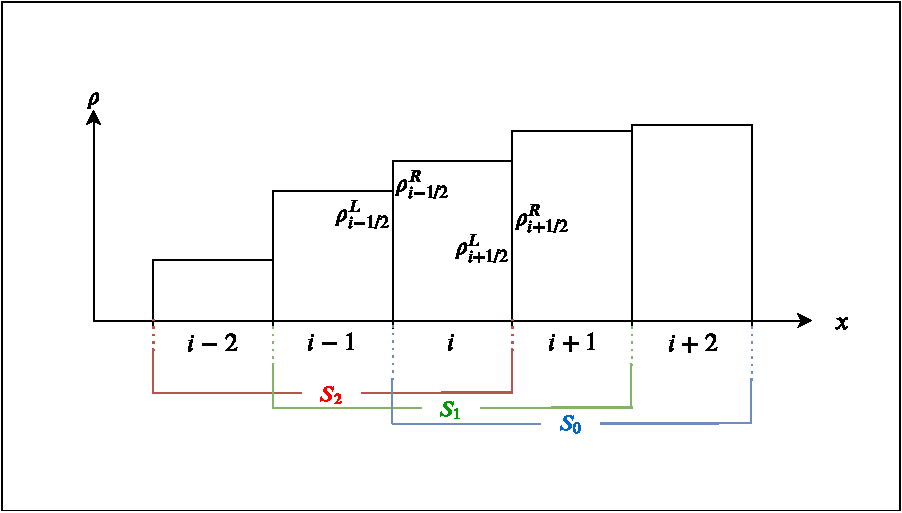
\includegraphics[trim=35 35 20 40,clip,width=\textwidth]{WENO5.pdf}
		\caption[WENO reconstruction stencil]{WENO stencil.}
		\label{fig:app:weno}
	\end{figure}
	
\subsection{Monotonicity Preserving Bounds}
\label{ap:monotonicitypreservingbounds}

	Proposing an improvement on Suresh and Huynh \cite{Suresh97}, Balsara and Shu \cite{BalsaraShu00} give a method to monotonically bound the reconstructed states. Suresh and Huynh \cite{Suresh97} found that bounding local extrema reduces the order of accuracy and should be avoided for higher order schemes. The following presents a scheme for the monotonicity preserving bound proposed in \cite{BalsaraShu00}. This method is applied to the $7^{th}$ order WENO reconstruction in Appendix \ref{code:wenoreconstruction}. Begin by defining the minmod and median functions,
	\begin{align}	
		\mathrm{minmod}(x,y)&=\frac{1}{2}\left(\mathrm{sign}(x)+\mathrm{sign}(y)\right)\min\left(|x|,|y|\right),\\
		\mathrm{median}(x,y,z)&=x+\mathrm{minmod}(y-x,z-x).
	\end{align}
	In alignment with the the substeps $a$ to $e$ of step 7 in the WENO code in Appendix \ref{code:wenoreconstruction}, step $7a$ defines the local curvature measures $d_j,d_{j+1},d_{j-1}$ similarly by
	\begin{equation}
		d_j=\rho_{j+1}-2\rho_{j}+\rho_{j-1}.
	\end{equation}
	Step $7b$ improves on Suresh and Huynh \cite{Suresh97} by taking the minmod, allowing local extrema to develop,
	\begin{equation}
		\rho_{j+1/2}^{MM}=\mathrm{minmod}(d_j,d_{j+1}).
	\end{equation}
	As well as the minmod evaluation (denoted in the superscript $MM$), an allowance is made for large curvature ($LC$) controlled by the parameter $\beta$. Step $7c$ defines $\beta$ and $\alpha$ two curvature constant parameters. The value of $\beta$ determines the freedom from allowing a large local curvature , and $\alpha$ determines the appropriate CFL number. Suresh and Huynh \cite{Suresh97} claim setting $\alpha=2$ and $\beta=4$ allow a CFL of at least 0.6 and do not degrade the monotonicity preserving property. Step $7d$ define the median ($MD$), upper limit ($UL$) and large curvature ($LC$) density solutions. The following provide definitions for the right states, the left can be evaluated symmetrically,
	\begin{align}
		\rho_{j+1/2}^{MD}&=\frac{1}{2}\left(\rho_j+\rho_{j+1}\right)-\frac{1}{2}d_{j+1/2}^{MD},\\
		\rho_{j+1/2}^{UL}&=\rho_j+\alpha\left(\rho_j-\rho_{j-1}\right),\\
		\rho_{j+1/2}^{LC}&=\rho_j+\frac{1}{2}\left(\rho_j-\rho_{j-1}\right)+\frac{\beta}{3}d_{j-1/2}^{LC}.
	\end{align}
	Step $7e$ defines new bounds for the maximum and minimum reconstructed states before computing the monotonicity preserving value.
	\begin{align}
		\rho_{j+1/2}^{L,\min}&=\max\left\{\min\left(\rho_j,\rho_{j+1},\rho_{j+1/2}^{MD}\right),\min\left(\rho_j,\rho_{j+1/2}^{UL},\rho_{j+1/2}^{LC}\right)\right\},\\
		\rho_{j+1/2}^{L,\max}&=\min\left\{\max\left(\rho_j,\rho_{j+1},\rho_{j+1/2}^{MD}\right),\max\left(\rho_j,\rho_{j+1/2}^{UL},\rho_{j+1/2}^{LC}\right)\right\}.
	\end{align}
	Finally the monotonicity preserving bounds are calculated and returned as outputs of the WENO function,
	\begin{equation}
		\rho_{j+1/2}^L=\mathrm{median}(\rho^L_{j+1/2},\rho^{L,\min}_{j+1/2},\rho^{L,\max}_{j+1/2}).
	\end{equation}
	Within this approach there are many outcomes achieved by setting $d^{MD}$, $d^{LC}$, $d^{MM}$ equal in various combinations. The paper from Balsara and Shu \cite{BalsaraShu00} tests these monotonicity preserving bounds on standard hyperbolic test cases. 
	












